% SSU Data Dash 2026: team report template. Compile from this folder (Overleaf: upload the whole
% repository as a zip). `python run.py report` writes the results table and figure it includes.
% Keep the report to 4 pages, not counting the outside-data table and the appendix.
\documentclass[11pt]{article}
\usepackage[margin=2.2cm]{geometry}
\usepackage{graphicx,booktabs,hyperref}
\usepackage{amsmath}
\graphicspath{{../figures/}}
\setlength{\parskip}{4pt}

% Required: your team name and the full name of every team member.
\title{SSU Data Dash 2026: \textit{The Outlier}}
\author{\textit{Wenjun Bo, Maggie Huang, Tianyi Zhao, Yibo Zhang}}
\date{}

\begin{document}
\maketitle

\noindent\begin{tabular}{@{}ll}
\textbf{Video (YouTube, unlisted is fine):} & \url{https://youtu.be/d42YsT9QbvA} \\
\textbf{Code and submission files (GitHub):} & \url{https://github.com/1mmagg1e/DATA-DASH-2026} \\
\end{tabular}

\section*{Summary}
% Three or four sentences: your approach, your validation result, and your main finding.
We predict simulated Toronto home sale prices using Box--Cox multiple linear regression for the off-market track and Ridge regression and an area spline for the list-aware track. Both models use the preceding 12 months of sales. Monthly walk-forward validation from December 2025 to May 2026 yields pooled MdAPE of 11.746\% off-market and 4.453\% list-aware. Restricting training to recent sales produced a much larger list-aware improvement than adding further location or lot variables; access to list price is associated with substantially lower prediction errors.

\section{Data and features}
% Which columns you used, what you built from them, and anything you dropped and why.
We use only the supplied synthetic competition dataset, \href{https://huggingface.co/datasets/Baliyang/SSU_data_dash}{Baliyang/SSU\_data\_dash}, with training sales available through May 2026. Both tracks use bedrooms, washrooms, total parking, house-area midpoint, property type and house style. House-area ranges are represented by their midpoints. Missing numerical values use training medians; categorical inputs are one-hot encoded, with unseen categories ignored at prediction time.

Off-market adds municipality, community, lot frontage and lot depth, including indicators for missing lot dimensions. Missing categorical values use the most frequent training category. List-aware adds list price and a combined municipality--community identifier to distinguish similarly named communities. Missing identifier components receive an ``Unknown'' label; property type and style use most-frequent imputation. Separate municipality indicators and lot dimensions are not included in the final list-aware specification.

Sold price is our training target, not include as an input. Sale date is used to define training window and validation folds only. Neither model uses days on market or external AVM estimates, off-market also excludes list price from training model. All learned preprocessing, including medians, scaling, transformations and spline knots, is fitted within each training window.


\section{Models}
% One paragraph per track. Off-market has no list price; list-aware does. Explain how your two
% models differ and why.


\textbf{Off-market.} We use Ordinary least squares predicts Box--Cox-transformed sale price. Bedrooms, washrooms, parking and area also get Box--Cox transformations; the three count variables are shifted by one first to handle zeros. Transformation parameters are estimated using training data. Transformed predictors and median-imputed lot dimensions are standardized; missing-lot indicators enter directly. Predictions return to dollars through direct inverse Box--Cox transformation, without smearing correction. The final model uses a 12-month training window and lot features, without lot interactions or a listing-time trend.

\textbf{List-aware.} Ridge regression fits sale price in dollars with penalty $\alpha=100$, standardized numerical predictors and categorical indicators. House-area midpoint enters through a cubic spline with four training-quantile knots, no bias basis and linear extrapolation. Spline features are standardized. This allows a flexible area--price relationship while remaining linear in the fitted coefficients. The final specification uses community features and a 12-month training window.


\section{Validation}
% How you tested the models without using information from the future: which months you
% trained on, which you predicted, and how you made sure nothing leaked.
For each of six validation months (December 2025--May 2026), a fresh model is trained on sales in $[t-12\text{ months},t)$, where $t$ is the first day of that month. It predicts sale prices for homes in the validation month, excluding target-related fields from the predictors. Each track has 10,069 validation predictions. Dollar predictions are rounded once before scoring. Absolute percentage error is $100|\hat y_i-y_i|/y_i$; MdAPE is its median and MAPE its mean. Pooled metrics use all validation homes, rather than averaging monthly medians.

These months informed model selection, so the scores are development results rather than independent hidden-test performance. Final submission models are fitted on June 1, 2025--May 31, 2026 sales and remain fixed for all June--September 2026 test homes. Unlike monthly validation, this protocol does not refit using later sale labels.

\section{Results}
\begin{table}[h]
\centering
\begin{tabular}{lrccc}
\hline
Track & Homes & MdAPE \% (95\% CI) & MAPE \% (95\% CI) & Median signed error \% \\
\hline
off-market & 10,069 & 11.75 (11.48--12.05) & 14.95 (14.69--15.20) & +1.56 \\
list-aware & 10,069 & 4.45 (4.37--4.55) & 5.66 (5.57--5.75) & +0.79 \\
\hline
\end{tabular}
%% Written by `python run.py report`. Do not edit by hand: rerun the command instead.
\begin{tabular}{lrccc}
\hline
Track & Homes & MdAPE \% (95\% CI) & MAPE \% (95\% CI) & Median signed error \% \\
\hline
off-market & 10,069 & 11.75 (11.48--12.05) & 14.95 (14.69--15.20) & +1.56 \\
list-aware & 10,069 & 4.45 (4.37--4.55) & 5.66 (5.57--5.75) & +0.79 \\
\hline
\end{tabular}

\caption{Pooled walk-forward results, 10,069 homes per track. Positive signed error means overprediction. Bootstrap intervals resample individual homes.}
\end{table}
% Describe the numbers in words. What improved over the baselines, and by how much?
The original list-aware baseline achieved pooled MdAPE/MAPE of 6.670\%/7.650\%. Ridge with community features achieved 6.585\%/7.461\%; a 12-month window reduced these to 4.495\%/5.670\%. Adding the area spline yielded 4.453\%/5.656\%, a further 0.042 percentage-point MdAPE reduction. Final MdAPE is 2.217 percentage points below the original baseline. The spline improved monthly MdAPE in five of six months and monthly MAPE in all six. Adding municipality and lot features to the spline model slightly worsened pooled MdAPE/MAPE to 4.456\%/5.658\%, so we retained the simpler specification.

Off-market, adding lot features to the 12-month Box--Cox model reduced pooled MdAPE from 11.953\% to 11.746\% and MAPE from 15.122\% to 14.945\%. Lot interactions yielded 11.779\%/14.947\%, offering no pooled advantage. These small feature gains are descriptive; we do not claim statistical significance. The gap between tracks is consistent with list price supplying information absent from structural and location features, but is not a controlled causal estimate of its contribution.


\section{Where the model fails}
\begin{figure}[h]
\centering
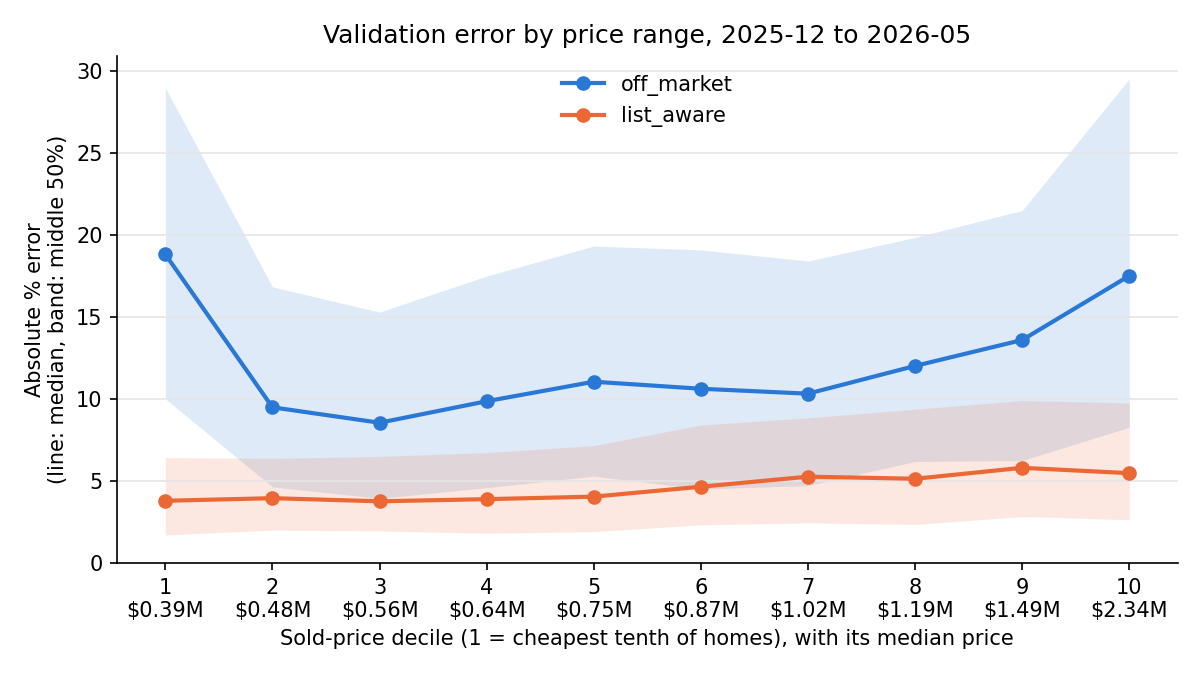
\includegraphics[width=0.85\linewidth]{error_by_price_range.png}
\caption{Validation error by actual sold-price decile. Lines show median absolute percentage error; bands show the middle 50\% of errors, not confidence intervals.}
\end{figure}
% Add your own breakdowns: by month, property type, neighbourhood, size.
Off-market errors are greatest at the price extremes: median absolute percentage error is approximately 19\% in the cheapest decile and 17\% in the most expensive, versus about 9--11\% across several middle deciles. Percentage error is sensitive to small price denominators, while expensive homes may have attributes absent from the available features. These are plausible explanations, not established causes. List-aware median errors remain around 4--6\% across deciles, with wider dispersion among expensive homes. Sold-price deciles are used only for retrospective diagnosis, never as prediction inputs.

Monthly off-market MdAPE ranges from 10.935\% in March to 13.751\% in December; list-aware MdAPE ranges from 4.329\% in December to 4.671\% in February. Aggregate results therefore conceal temporal variation. Positive median signed errors of 1.56\% and 0.79\% indicate residual overprediction, but do not imply every home or subgroup is overpredicted.

\section{Limitations}

Synthetic-data results do not establish performance on real Toronto transactions. Repeated validation reuse can make selected-model estimates optimistic; individual-home bootstrap intervals do not capture shared market shocks or selection uncertainty. Using a recent training window excludes older observations and can leave sparse communities less well represented. Ignoring unseen categories permits prediction without learning their local price effects. Area midpoints lose within-range variation, and direct inverse Box--Cox predictions need not estimate mean dollar price without retransformation adjustment.

The fixed final model may become less accurate later in the test period as conditions change. A useful next evaluation would reserve an untouched four-month period with a fixed training cutoff, matching deployment, and examine errors in sparse communities and price extremes. Hidden-test labels are unavailable: submission checks establish format validity, not accuracy.

\section*{Outside data}
% Every outside source, or write "None". Data may only cover periods up to and including May 2026.
\begin{tabular}{lll}
\toprule
Source & URL & Periods covered \\
\midrule
\textit{None} & & \\
\bottomrule
\end{tabular}

\section*{Reproducing our results}
% The exact commands that produce your two submission files from a fresh copy of your repository.
From the GitHub repository root, in a Python 3.13 environment:
\begin{verbatim}
pip install -r requirements.txt
python run.py validate
python run.py report
python verify_final_models.py
python run.py predict
python run.py check
\end{verbatim}
The loader downloads official data by default; alternatively, set \texttt{DATA\_DIR} to the folder containing the official training and test CSVs. 

The files \texttt{submissions/submission\_off\_market.csv} and \texttt{submissions/submission\_list\_aware.csv} contain 3,974 and 4,064 predictions respectively, with columns \texttt{ml\_num} and \texttt{predicted\_price}. 

Both passed official ID, column and positive-finite-value checks locally. Validation and prediction were reproduced with local CSVs and the packaged code; a clean-environment installation and automatic-download route have not yet been independently verified.
\end{document}